\documentclass{article}
\usepackage{graphicx}
\graphicspath{{../images/}}
\title{First document}
\author{Hubert Farnsworth \thanks{funded by the Overleaf team}}
\date{\today}
\begin{document}
	\begin{abstract}
		This is a simple paragraph at the beginning of the 
		document. A brief introduction about the main subject.
	\end{abstract}


	\tableofcontents

	\section{LOL}
	The universe is immense and it seems to be homogeneous, 
	in a large scale, everywhere we look at.
	
	%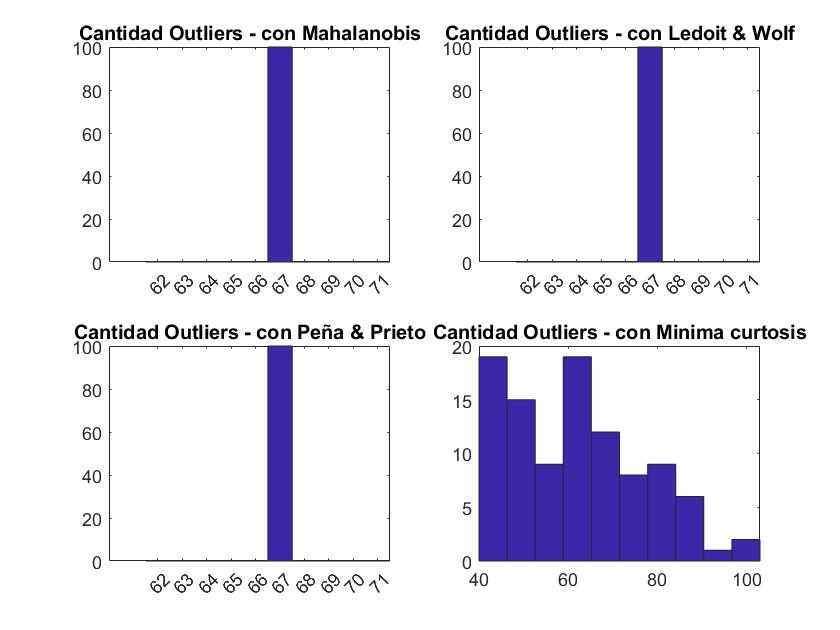
\includegraphics{comp7} %include image
	
	There's a picture of a galaxy above
	Some of the greatest \emph{discoveries} 
	in science 
	were made by accident.
	
	\textit{Some of the greatest \emph{discoveries} 
		in science 
		were made by accident.}
	
	\textbf{Some of the greatest \emph{discoveries} 
		in science 
		were made by accident.}
	\begin{figure}[h]
		\centering
		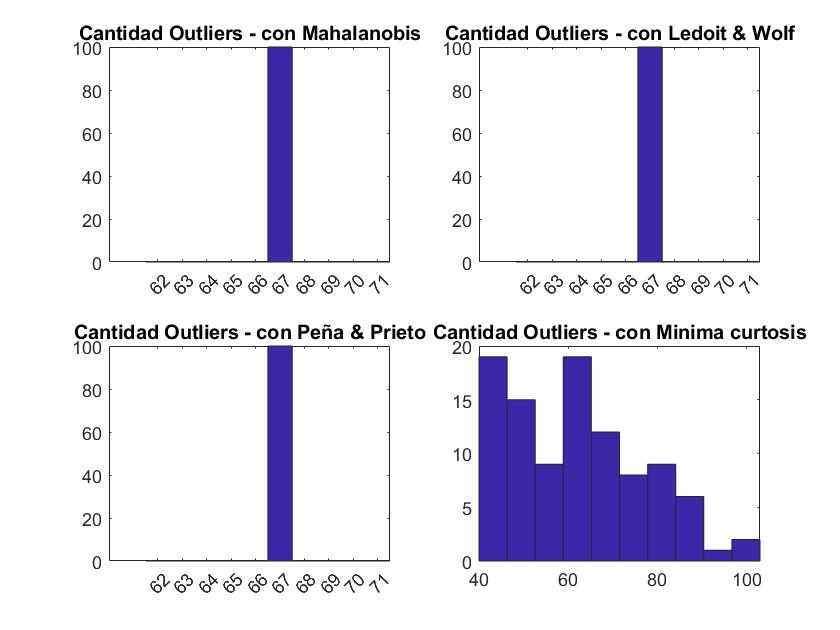
\includegraphics[width=0.25\textwidth]{comp7}
		\caption{a nice plot}
		\label{fig:mesh1}
	\end{figure}
	In physics, the mass-energy equivalence is stated 
	by the equation $E=mc^2$, discovered in 1905 by Albert Einstein.
%	\chapter{First Chapter}
	
	\section{Introduction}
	
	This is the first section.
	
	Lorem  ipsum  dolor  sit  amet,  consectetuer  adipiscing  
	elit.   Etiam  lobortisfacilisis sem.  Nullam nec mi et 
	neque pharetra sollicitudin.  Praesent imperdietmi nec ante. 
	Donec ullamcorper, felis non sodales...
	
	$\frac{12}{13}*\sqrt{X^{2}}$
	
	\section{Second Section}
	
	Lorem ipsum dolor sit amet, consectetuer adipiscing elit.  
	Etiam lobortis facilisissem.  Nullam nec mi et neque pharetra 
	sollicitudin.  Praesent imperdiet mi necante...
	
	\subsection{First Subsection}
	Praesent imperdietmi nec ante. Donec ullamcorper, felis non sodales...
	
	\section*{Unnumbered Section}
	Lorem ipsum dolor sit amet, consectetuer adipiscing elit.  
	Etiam lobortis facilisissem
	
	%table
	\begin{center}
		\begin{tabular}{ c c c }
			cell1 & cell2 & cell3 \\ 
			cell4 & cell5 & cell6 \\  
			cell7 & cell8 & cell9    
		\end{tabular}
	\end{center}
    %With borders
    \begin{center}
    	\begin{tabular}{ |c|c|c| } 
    		\hline
    		cell1 & cell2 & cell3 \\ 
    		cell4 & cell5 & cell6 \\ 
    		cell7 & cell8 & cell9 \\ 
    		\hline
    	\end{tabular}
    \end{center}
	\begin{center}
		\begin{tabular}{||c c c c||} 
			\hline
			Col1 & Col2 & Col2 & Col3 \\ [0.5ex] 
			\hline\hline
			1 & 6 & 87837 & 787 \\ 
			\hline
			2 & 7 & 78 & 5415 \\
			\hline
			3 & 545 & 778 & 7507 \\
			\hline
			4 & 545 & 18744 & 7560 \\
			\hline
			5 & 88 & 788 & 6344 \\ [1ex] 
			\hline
		\end{tabular}
	\end{center}
	Table \ref{table:data} is an example of referenced \LaTeX{} elements.
	
	\begin{table}[h!]
		\centering
		\begin{tabular}{||c c c c||} 
			\hline
			Col1 & Col2 & Col2 & Col3 \\ [0.5ex] 
			\hline\hline
			1 & 6 & 87837 & 787 \\ 
			2 & 7 & 78 & 5415 \\
			3 & 545 & 778 & 7507 \\
			4 & 545 & 18744 & 7560 \\
			5 & 88 & 788 & 6344 \\ [1ex] 
			\hline
		\end{tabular}
		\caption{Table to test captions and labels}
		\label{table:data}
	\end{table}
\end{document}